\documentclass{beamer}

\usepackage[sfdefault]{cabin}
\usepackage[utf8]{inputenc}
\usepackage[T1]{fontenc}
\usepackage[french]{babel}
\usepackage{xcolor}
\usepackage{caption}
\usepackage{graphicx}
\usepackage{multicol}
%Police
%\usepackage[sfdefault]{roboto}
\usepackage[sfdefault]{FiraSans}

\definecolor{modernblue}{RGB}{70,130,180} 
\definecolor{modernvert}{RGB}{0, 80, 0}
\definecolor{sparkorange}{RGB}{237,127,16} 

\usetheme{Madrid}

\usecolortheme[named=sparkorange]{structure}

\setbeamertemplate{caption}{\insertcaption} % Utiliser le format de légende par défaut de Beamer



\renewcommand{\thesection}{\Roman{section}}\renewcommand{\thesubsection}{\arabic{subsection} }\renewcommand{\thesubsubsection}{\alph{subsubsection} }

\newcommand{\C}{\mathbb{C}}\newcommand{\R}{\mathbb{R}}\newcommand{\Q}{\mathbb{Q}}\newcommand{\Z}{\mathbb{Z}}\newcommand{\N}{\mathbb{N}}\newcommand{\V}{\overrightarrow}\newcommand{\Cs}{\mathscr{C}}\newcommand{\Ps}{\mathscr{P}}\newcommand{\Rs}{\mathscr{R}}\newcommand{\Gs}{\mathscr{G}}\newcommand{\Ds}{\mathscr{D}}\newcommand{\happy}{\huge\smiley}\newcommand{\sad}{\huge\frownie}\newcommand{\alors}{\Large\Rightarrow}\newcommand{\equi}{\Leftrightarrow}
\newcommand{\disp}{\displaystyle}\newcommand{\Pro}{\mathbb{P}}


\newtheorem{thm}{Théorème}
\newtheorem{rmq}{Remarque}
\newtheorem{prop}{Propriété}
\newtheorem{cor}{Corollaire}
\newtheorem{lem}{Lemme}
\newtheorem{prop-def}{Propriété-définition}

\theoremstyle{definition}

\newtheorem{defi}{Définition}
\newtheorem{intro}{Introduction :}
\def\di{\displaystyle}

\title{Accidents de la circulation en France}
\date{6 Décembre 2023}
\author{Ivanhoé Botcazou}

\begin{document}
	
\begin{frame}[plain]
    \maketitle
   	\begin{figure}
   	
\includegraphics[scale=0.5]{spark.png}
	\end{figure}
\end{frame}



%FRAME
\begin{frame}[plain]

\begin{figure}
	\begin{intro}
		\par Les données misent à notre disposition sont des tableaux au format 'csv'. Nous retrouvons par année différentes modalités sur les accidents de la circulation routière : caractéristiques, usagers, lieux et véhicules. Nous chercherons à répondre aux questions suivantes :
	\end{intro}
\begin{itemize}
	\item Quelle est l'évolution du nombre d'accidents de la circulation en France par année ?
	\item Y a-t-il une zone géographique française plus touchée par les accidents de la circulation ?
	\item Le niveau d'éclairage au moment de l'accident est-il un facteur aggravant ?
	\item Quelle est l'évolution du nombre de morts et de blessés sur la route en France par année ?
	\item Quelles sont les 10 catégories de véhicules les plus meurtrières sur ces années pour les conducteurs ?
	\item Quelle classe d'âge est la plus touchée dans des accidents meurtriers sur la route ?
\end{itemize}
	
\end{figure}
\end{frame}

%FRAME
\begin{frame}
	\frametitle{Évolution du nombre d'accidents de la circulation en France par année}
	\centering
	\begin{minipage}[c]{0.8\linewidth}\centering\begin{figure}

				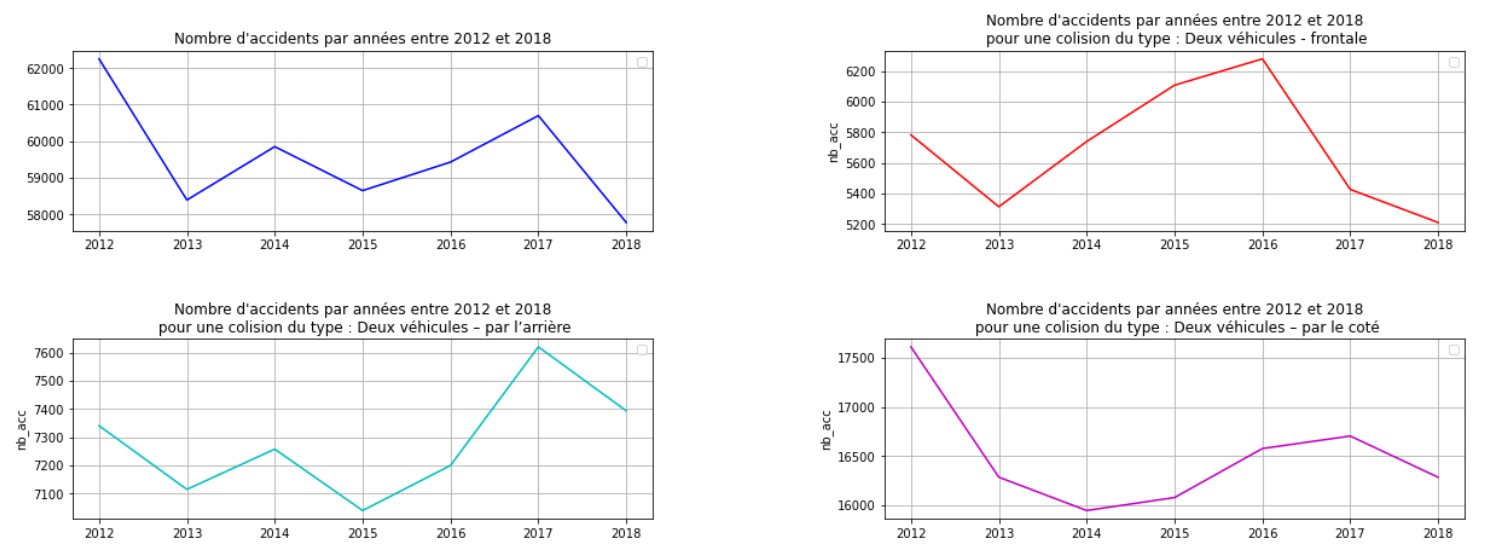
\includegraphics[width=1\linewidth]{evo1.png}
		\end{figure}
	\end{minipage}
	
		\begin{minipage}[t]{0.8\linewidth}\centering\begin{figure}
				\begin{center}
					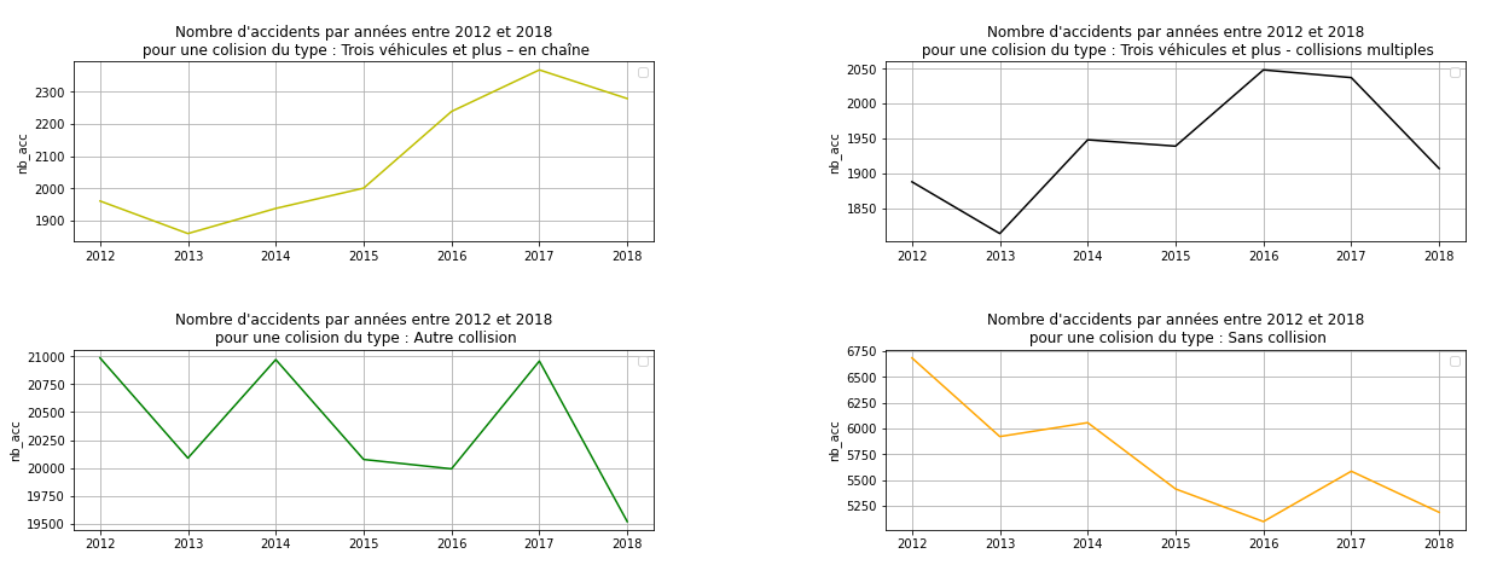
\includegraphics[width=1\linewidth]{evo2.png}			
				\end{center}
				
		\end{figure}\end{minipage}	
\end{frame}

%FRAME
\begin{frame}
	\frametitle{Zones géographiques françaises et accidents de la circulation}
	La France est partagée en 6 parties distinctes entre le nord, le sud, l'ouest, l'est et le centre(NO,NC,NE,SO,SC,SE). Approximativement, les villes repères pour la longitude sont Le Mans et Reims, la ville repère pour la latitude est Bourge.\\[0.5cm]
	\begin{minipage}[c]{1\linewidth}
		\begin{minipage}[t]{0.48\linewidth}\centering\begin{figure}
				\centering
				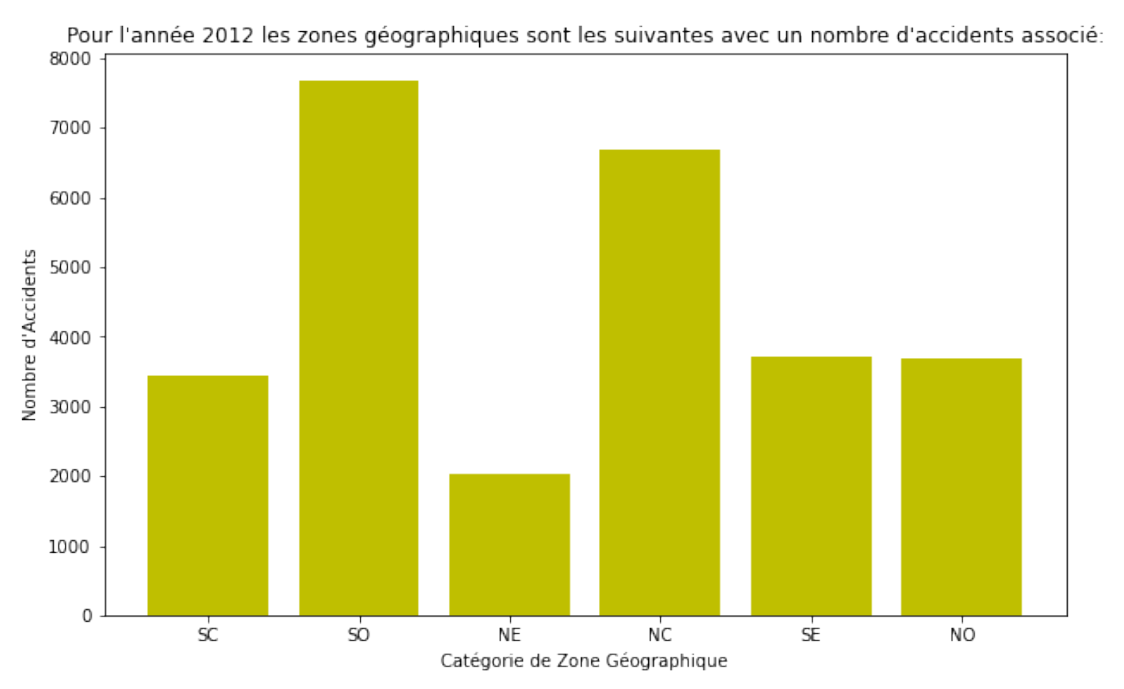
\includegraphics[width=1\linewidth]{geo1.png}
		\end{figure}\end{minipage}\hfill 
		\begin{minipage}[t]{0.48\linewidth}\centering\begin{figure}
				\begin{center}
					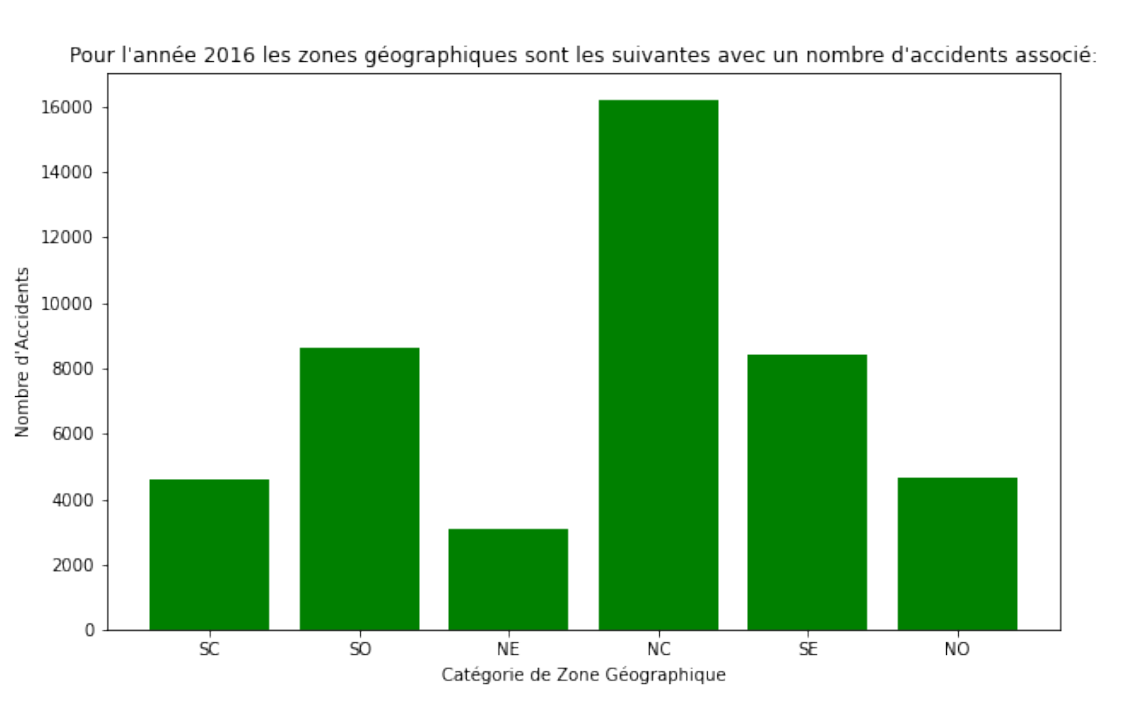
\includegraphics[width=1\linewidth]{geo2.png}			
				\end{center}
				
		\end{figure}\end{minipage}
	\end{minipage}
	
	
\end{frame}

\begin{frame}
	\frametitle{Niveau d'éclairage au moment de l'accident}

	\begin{minipage}[t]{1\linewidth}
		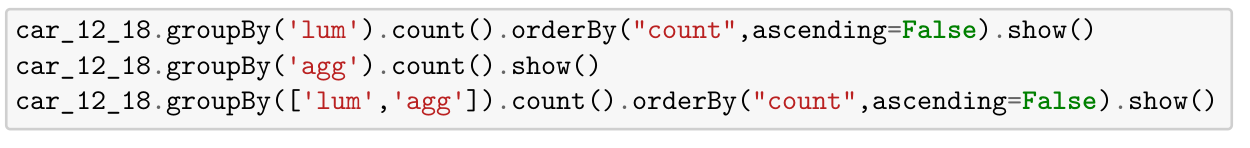
\includegraphics[width=1\linewidth]{lum0.png}
		\begin{minipage}[t]{0.3\linewidth}\centering\begin{figure}
				\centering
				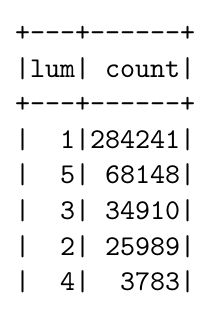
\includegraphics[width=1\linewidth]{lum1.png}
		\end{figure}\end{minipage}\hfil 
		\begin{minipage}[t]{0.3\linewidth}\centering\begin{figure}
				\begin{center}
					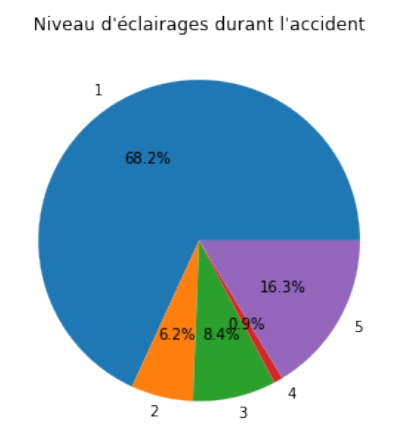
\includegraphics[width=1\linewidth]{lum4.png}			
				\end{center}
			\end{figure}\end{minipage}\hfil
		\begin{minipage}[t]{0.3\linewidth}\centering\begin{figure}
				\begin{center}
					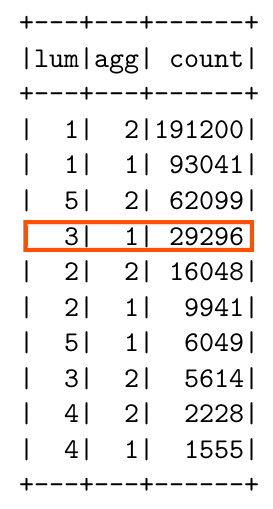
\includegraphics[width=1\linewidth]{lum3.png}			
				\end{center}
				
		\end{figure}\end{minipage}

	\end{minipage}	
	
\end{frame}

\begin{frame}
	\frametitle{Accident à la campagne de nuit}
	
	\begin{minipage}[t]{1\linewidth}
		\centering
		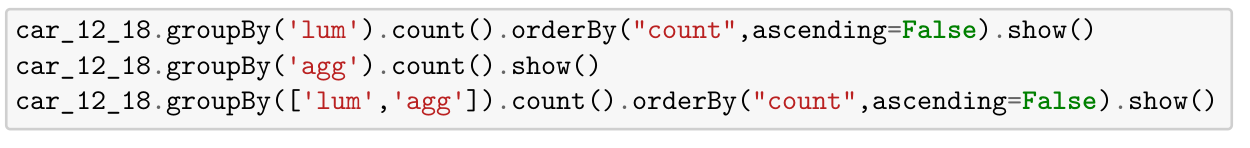
\includegraphics[width=1\linewidth]{lum0.png}\\[-0.25cm]
		\begin{minipage}[t]{0.48\linewidth}\centering\begin{figure}
				\raggedright
				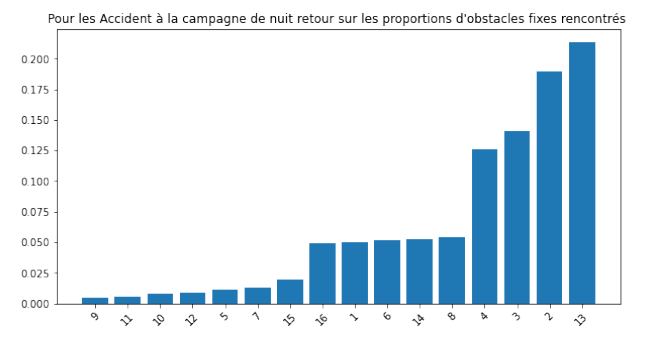
\includegraphics[width=1\linewidth]{camp1.png}
				\begin{enumerate}
					\item[13.] Fossé, talus, paroi rocheuse
					\item[2.] Arbre
					\item[3.] Glissière métallique
					\item[4.] Glissière béton
				\end{enumerate}
		\end{figure}\end{minipage}\hfil 
		\begin{minipage}[t]{0.48\linewidth}\centering\begin{figure}
				\raggedright
				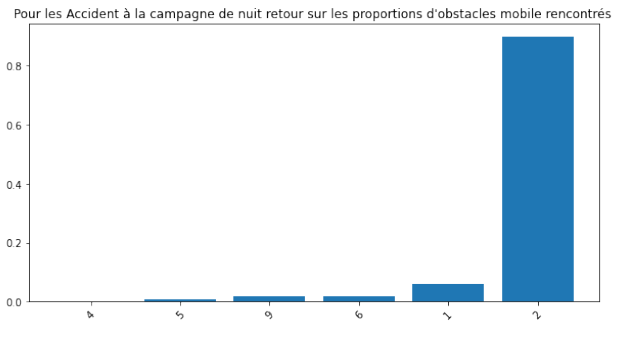
\includegraphics[width=1\linewidth]{camp2.png}
				\begin{enumerate}
					\item[2.] Véhicule
					\item[1.] Piéton
					\item[6.] Animal sauvage
					\item[9.] Autre
				\end{enumerate}		
				
		\end{figure}\end{minipage}
		
	\end{minipage}	
	
\end{frame}

%FRAME
\begin{frame}
	\frametitle{Morts et de blessés sur la route en France par année}
	\centering
	\begin{minipage}[c]{1\linewidth}\centering\begin{figure}
			
			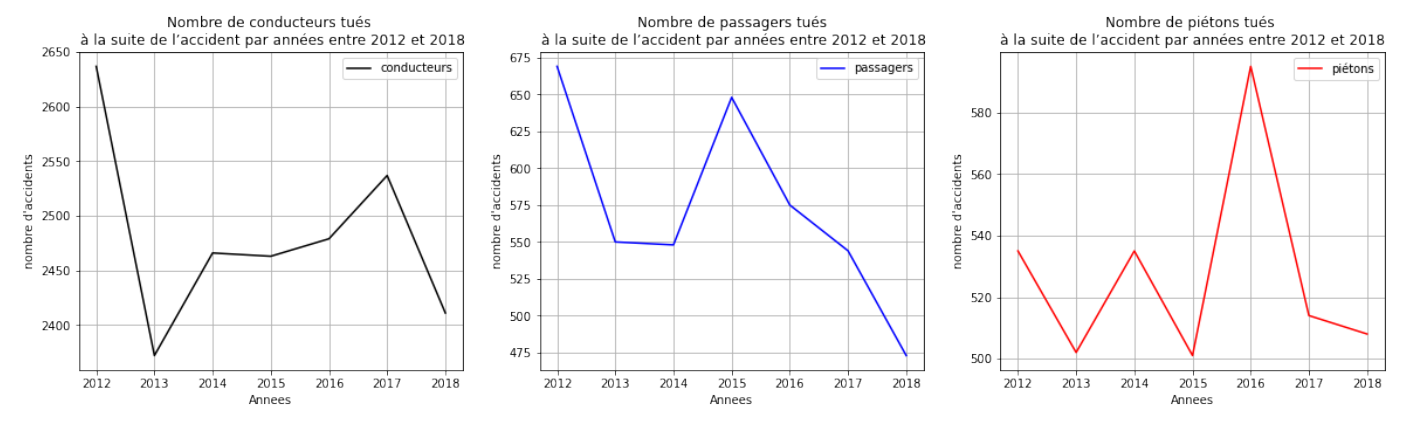
\includegraphics[width=1\linewidth]{morts.png}
		\end{figure}
	\end{minipage}
	
	\begin{minipage}[t]{1\linewidth}\centering\begin{figure}
			\begin{center}
				\includegraphics[width=1\linewidth]{blessés.png}			
			\end{center}
			
	\end{figure}\end{minipage}	
\end{frame}

%FRAME
\begin{frame}
	\frametitle{Morts sur la route en France entre 2012 et 2018}
	\centering
	\begin{minipage}[c]{1\linewidth}\centering\begin{figure}
			
			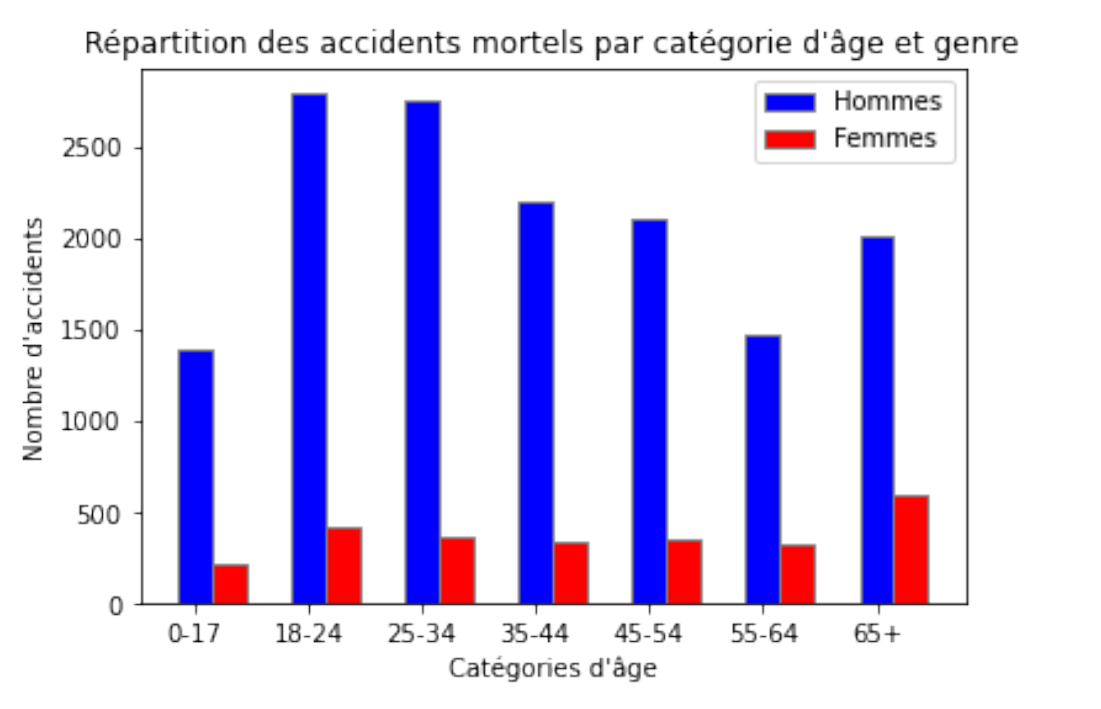
\includegraphics[width=1\linewidth]{morts_genre.png}
		\end{figure}
	\end{minipage}
	
\end{frame}

%FRAME
\begin{frame}
	\frametitle{Véhicules les plus meurtriers entre 2012 et 2018}
	\centering
	\begin{minipage}[c]{1\linewidth}\centering\begin{figure}
			
			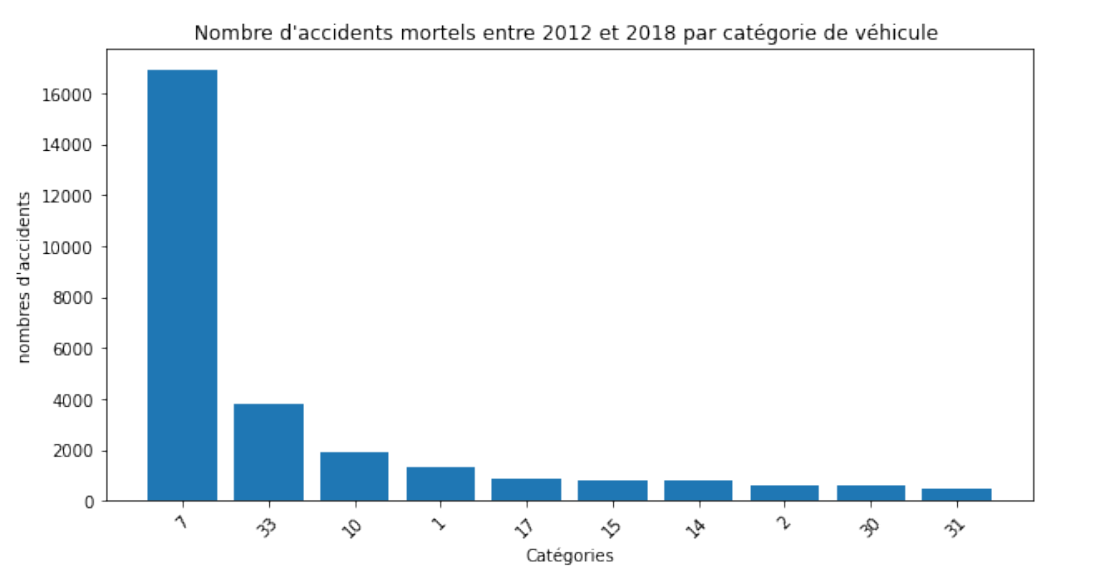
\includegraphics[width=0.8\linewidth]{vehicules.png}
		\end{figure}
	\end{minipage}
	\begin{minipage}[c]{1\linewidth}\centering\begin{figure}
			\begin{multicols}{2}
				\begin{enumerate}
					\item[7.] VL seul, (véhicules légers inférieur ou égal à 3,5 tonnes)
					\item[33.] Motocyclette > 125 cm3
					\item[10.] VU seul 1,5T <= PTAC <= 3,5T avec ou sans remorque 
					\item[1.] Bicyclette
				\end{enumerate}	
			\end{multicols}
		
		
	\end{figure}
\end{minipage}
	
\end{frame}


\end{document}








